\documentclass[11pt]{article}
\usepackage{fullpage}
\usepackage{graphics,epsfig,color}
\usepackage{wrapfig}
\usepackage{times}
\usepackage{setspace}
\usepackage{amsmath,amsthm,amssymb}
\usepackage{url}
\usepackage{fancyhdr}
\usepackage{enumitem}

\pagestyle{fancy}


\newtheorem{theorem}{Theorem}[section]
\newtheorem{corollary}{Corollary}[section]
\newtheorem{lemma}{Lemma}[section]
\newtheorem{problem}{Problem}
\newtheorem{definition}{Definition}[section]
\newtheorem{observation}{Observation}[section]
\newtheorem{example}{Example}[section]
\newtheorem{openproblem}{Open Problem}[section]
\newtheorem{fact}{Fact}[section]

\newcommand{\qedsymb}{\hfill{\rule{2mm}{2mm}}}
\newenvironment{proofsketch}
{
	\begin{trivlist}
	\item[\hspace{\labelsep}{\noindent Proof Sketch: }]
}{\qedsymb\end{trivlist}}



%the following few lines until usepackage{algorithm2e} is to avoid the
%conflicts of algorithm2e with other packages.
\makeatletter
\newif\if@restonecol
\makeatother
\let\algorithm\relax
\let\endalgorithm\relax
\usepackage[ruled,vlined,linesnumbered]{algorithm2e}

\newcommand{\remove}[1]{}



%--------------------------------


\begin{document}

	\renewcommand{\headrulewidth}{0.4pt}
	\setlength{\headheight}{38.0pt}
	\fancyhead[L]{\bf CSCD359 Homework 4, Winter 2012, 
	Eastern Washington University. Cheney, Washington. \\
	\bigskip Name: Eric Fode\hspace{40mm}EWU ID:00530214}


	\noindent{\bf Solution for Problem 1}\\
	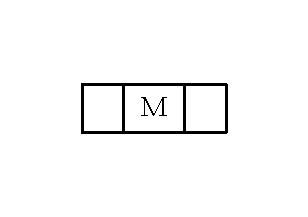
\includegraphics[scale=.5]{step1.pdf}
	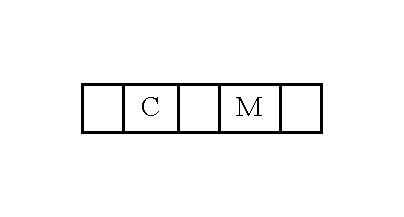
\includegraphics[scale=.5]{step2.pdf}
	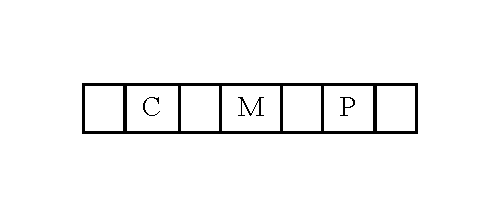
\includegraphics[scale=.5]{step3.pdf}
	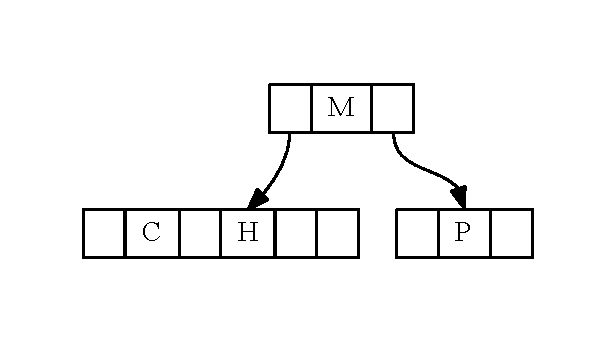
\includegraphics[scale=.5]{step4.pdf}\\
	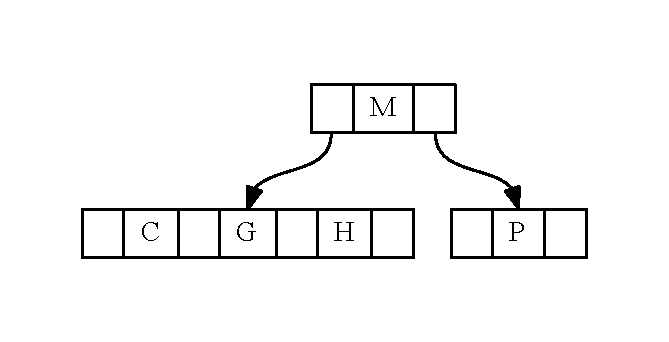
\includegraphics[scale=.5]{step5.pdf}
	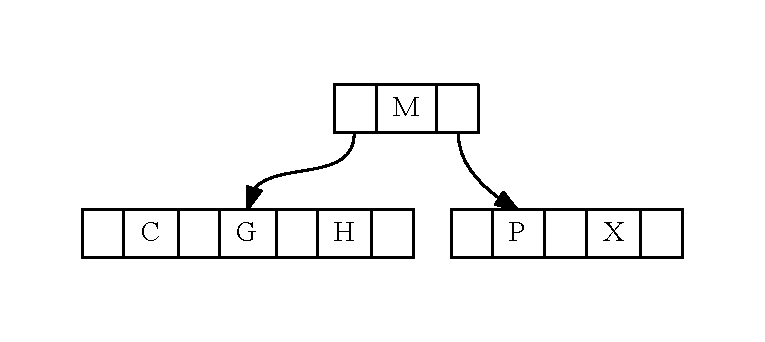
\includegraphics[scale=.5]{step6.pdf}\\
	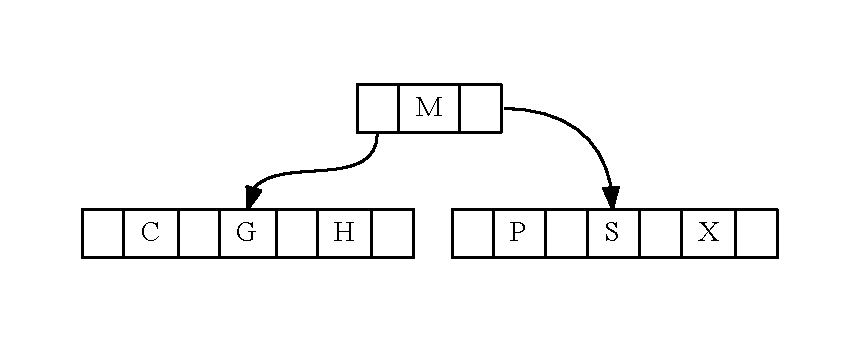
\includegraphics[scale=.5]{step7.pdf}
	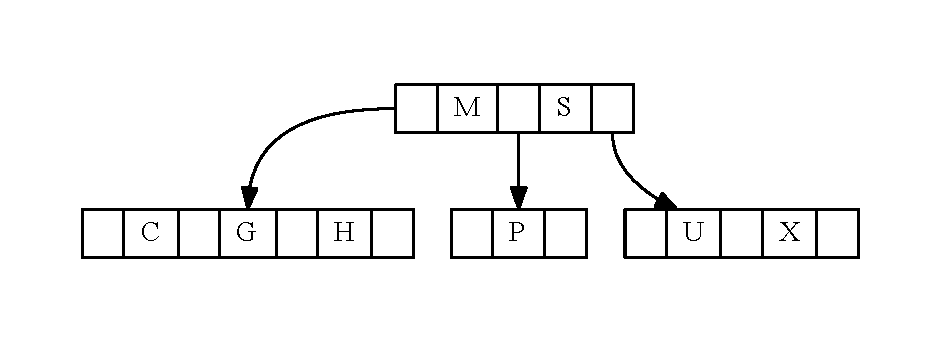
\includegraphics[scale=.5]{step8.pdf}\\
	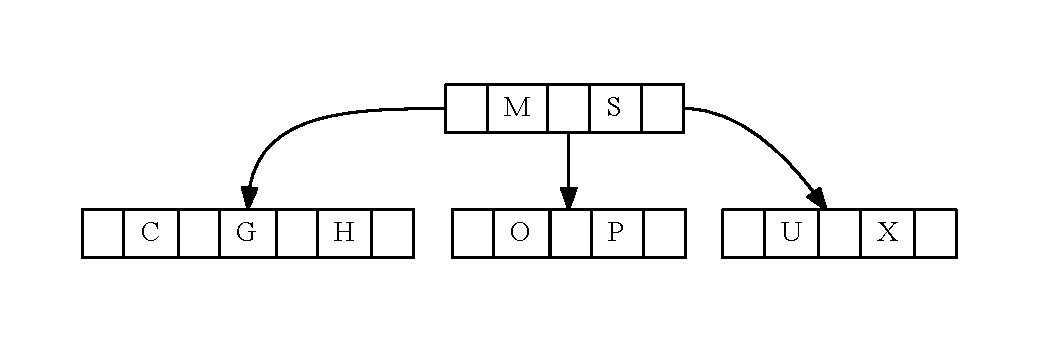
\includegraphics[scale=.5]{step9.pdf}\\
	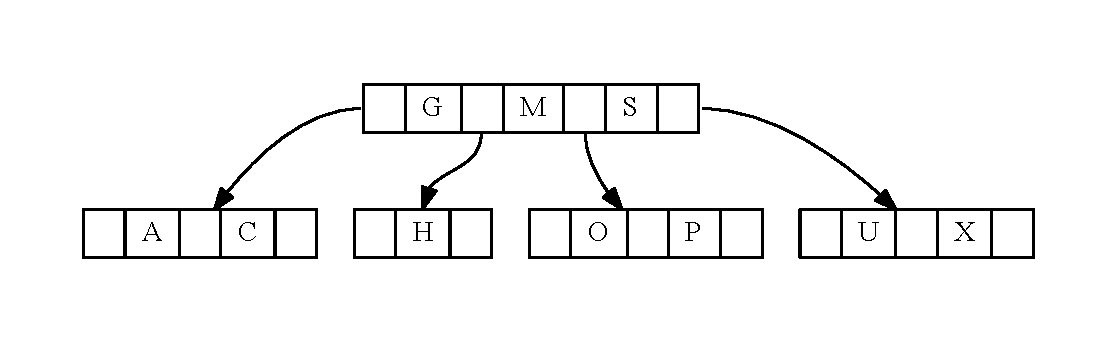
\includegraphics[scale=.5]{step10.pdf}\\
	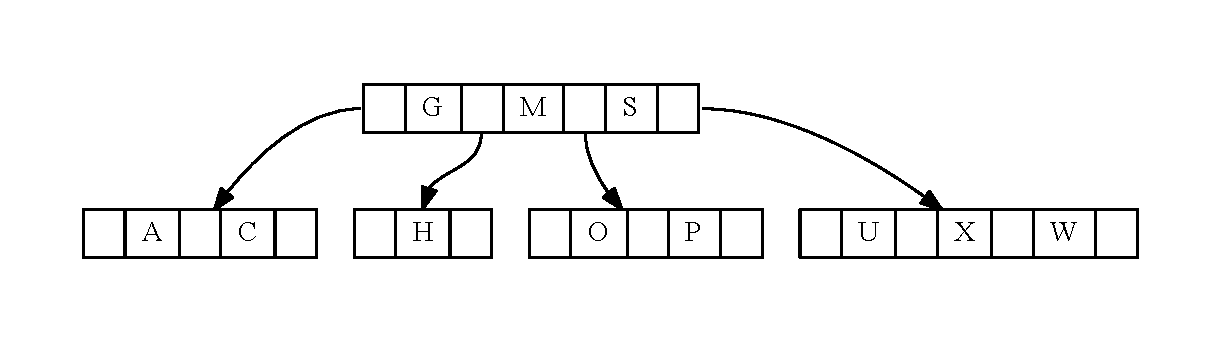
\includegraphics[scale=.5]{step11.pdf}
	
	\newpage
	
	\noindent{\bf Solution for Problem  2}\\
	
	\begin{algorithm}[H]
		\NoCaptionOfAlgo
		\caption{\bf sortedTree($treeArray$)}
		\KwIn{A slice of a sorted array}
		\KwResult{A BST that has a height bounded by $log(n)$}
		\Begin{
		
			\If{treeArray.size = 1}
			{
				\Return $new node(treeArray[0])$\;
			}
			$root = new node(treeArray[treeArray.size/2])$\;
			$root.left \longleftarrow sortedTree(treeArray[0:treeArray.size/2])$\;
			$root.right \longleftarrow sortedTree(treeArray[treeArray.size/2+1:treeArray.size])$\;
			\Return $root$\;
		}
		\end{algorithm}
	\noindent{\bf Analysis:} This should take $O(n)$ time
	\bigskip
	
	\noindent{\bf Solution for Problem 3}\\
	\bigskip
	
	\noindent{\bf Solution for Problem 4}\\
	
\end{document}